\documentclass[11pt, conference]{IEEEtran}
\usepackage{cite}
\usepackage{amsmath,amssymb,amsfonts}
\usepackage{algorithmic}
\usepackage{graphicx}
\usepackage{textcomp}
\usepackage{xcolor}
\usepackage{booktabs}
\usepackage{float}
\usepackage{hyperref}

\begin{document}

% --- Custom Title Page ---
\begin{titlepage}
    \centering
    \vspace*{0.3in}
    {\LARGE \bfseries COMPARATIVE ANALYSIS OF DEEP LEARNING ARCHITECTURES FOR BEAT-BY-BEAT ECG ARRHYTHMIA CLASSIFICATION \par}
    \vspace{0.8in}
    {\Large Interim report on \par}
    {\Large Deep Learning Project [ICT-4442] \par}
    \vspace{0.8in}
    {\Large \bfseries Submitted By \par}
    {\large Kotha Rusheel Reddy (230953176) \par}
    {\large Clarisha Lucia Pinto (230953112) \par}
    {\large Anshu S Malagi (230953196) \par}
    {\large Aaryan jaideep Kaneria (230953386) \par}
    \vspace{0.8in}
    
\includegraphics[width=1.8in]{manipal_logo.png} \par 
    \vspace{0.6in}
    {\large SCHOOL OF COMPUTER ENGINEERING \par}
    {\large MANIPAL INSTITUTE OF TECHNOLOGY, \par}
    {\large MANIPAL ACADEMY OF HIGHER EDUCATION \par}
    \vfill
    {\large October 2026 \par}
\end{titlepage}

% --- Header Info Page ---
\twocolumn[
\begin{center}
    \textbf{\Large PART B : INTERIM REPORT} \\
    \textbf{Phase 2} \\
    \vspace{0.5cm}
\end{center}
\textbf{Team No. and Names (with Registration Numbers):}
\begin{enumerate}
    \item Kotha Rusheel Reddy (230953176)
    \item Clarisha Lucia Pinto (230953112)
    \item Anshu S Malagi (230953196)
    \item Aaryan jaideep Kaneria (230953386)
\end{enumerate}
\vspace{0.3cm}
\textbf{Title of the Project:} A Comparative Analysis of Deep Learning Architectures for Beat-by-Beat ECG Arrhythmia Classification \\
\textbf{GitHub Repository Link:} \url{https://github.com/RK-0111/DL-project.git}
\vspace{0.8cm}
]

\section{Literature Review}
The automated detection of cardiac arrhythmias via Electrocardiogram (ECG) analysis has evolved significantly over the past two decades. Early methodologies, such as the seminal work by de Chazal et al. \cite{dechazal}, relied heavily on classical machine learning and manual feature engineering. Their research focused primarily on extracting RR intervals and manually tracking QRS morphology. Crucially, this paper established the foundational AAMI mapping standard and the DS1/DS2 inter-patient evaluation protocol that strictly segregates patients into separate sets to prevent data leakage. 

Despite this established protocol, Luz et al. \cite{luz} revealed a critical flaw in modern deep learning research. They demonstrated that many state-of-the-art models artificially inflate their classification accuracies to $>99\%$ by randomly splitting individual heartbeats across training and testing sets (known as intra-patient splitting). This allows models to memorize patient-specific baseline rhythms rather than generalizing to true pathological morphologies, strongly motivating our rigorous inter-patient testing pipeline. 

Furthermore, the extreme class imbalance in ambulatory ECGs presents a major challenge. In the MIT-BIH database, over $90\%$ of beats are entirely normal. This often causes neural networks to ignore rare, fatal ectopic beats in favor of majority-class accuracy. Sellami and Hwang \cite{sellami} addressed this via weighted loss algorithms, directly inspiring our implementation of the Synthetic Minority Oversampling Technique (SMOTE) to mathematically balance our dataset.

Architecturally, Kiranyaz et al. \cite{kiranyaz} proved that 1-Dimensional Convolutional Neural Networks (1D-CNNs) can automatically extract optimal spatial features without the need for manual engineering. Hannun et al. \cite{hannun} expanded this by utilizing deep 1D Residual Networks (ResNet) equipped with skip-connections, achieving cardiologist-level detection on massive ambulatory datasets. 

Conversely, Yildirim \cite{yildirim} demonstrated the unique efficacy of Bidirectional Long Short-Term Memory (BiLSTM) networks in capturing temporal rhythm contexts across sequences of heartbeats. Exploring hybrid models, Xia et al. \cite{xia} and Kachuee et al. \cite{kachuee} proved that cascading spatial CNN blocks into temporal LSTMs yields superior, highly transferable representations. Finally, Che et al. \cite{che} applied Transformer networks to ECG signals, evaluating self-attention mechanisms against traditional recurrent layers. Table \ref{tab:lit_review} summarizes these critical contributions.

\begin{table*}[t]
\centering
\caption{Literature Review Summary}
\label{tab:lit_review}
\begin{tabular}{|p{3.5cm}|p{3.5cm}|p{2cm}|p{4.5cm}|p{4cm}|}
\hline
\textbf{Paper (Author, Year)} & \textbf{Method} & \textbf{Dataset} & \textbf{Key Result} & \textbf{Relevance to Project} \\ \hline
de Chazal et al. (2004) \cite{dechazal} & Feature engineering & MIT-BIH & Established DS1/DS2 inter-patient protocol. & Defines core data-splitting methodology. \\ \hline
Luz et al. (2016) \cite{luz} & Survey of DL models & MIT-BIH & Showed random data splits artificially inflate accuracy. & Motivates our strict inter-patient split. \\ \hline
Kiranyaz et al. (2015) \cite{kiranyaz} & 1D-CNN & MIT-BIH & Proved CNNs automatically extract spatial ECG morphology. & Basis for ResNet and CNN-LSTM. \\ \hline
Sellami \& Hwang (2019) \cite{sellami} & CNN with weighted loss & MIT-BIH & Addressed severe class imbalance. & Informs SMOTE data augmentation. \\ \hline
Hannun et al. (2019) \cite{hannun} & 34-layer 1D ResNet & Ambulatory & Achieved cardiologist-level detection. & Validates 1D-ResNet architecture. \\ \hline
Yildirim (2018) \cite{yildirim} & Bidirectional LSTM & MIT-BIH & Proved LSTMs excel at temporal rhythm context. & Validates our recurrent hybrid block. \\ \hline
Kachuee et al. (2018) \cite{kachuee} & Transferable features & MIT-BIH & Explored generalizable architectures. & Reference for CNN-LSTM hybrid. \\ \hline
Xia et al. (2018) \cite{xia} & CNN-LSTM Hybrid & AFib Data & Combined spatial CNN and temporal LSTMs. & Matches our exact hybrid architecture. \\ \hline
Che et al. (2021) \cite{che} & Transformer Network & MIT-BIH & Applied self-attention to ECG signals. & Backing for 1D Vision Transformer. \\ \hline
\end{tabular}
\end{table*}

\section{Dataset Acquisition \& Preprocessing}
We utilize the internationally recognized MIT-BIH Arrhythmia Database accessed via PhysioNet. The corpus contains 48 ambulatory Holter ECG recordings (30 minutes each), encompassing over 100,000 expertly annotated heartbeats. The 2-channel physiological signals are sampled at a frequency of 360 Hz. The raw expert annotations were computationally aggregated into the standard five Association for the Advancement of Medical Instrumentation (AAMI) super-classes: Normal (N), Supraventricular (S), Ventricular (V), Fusion (F), and Unknown/Paced (Q). 

\begin{figure}[H]
    \centering
    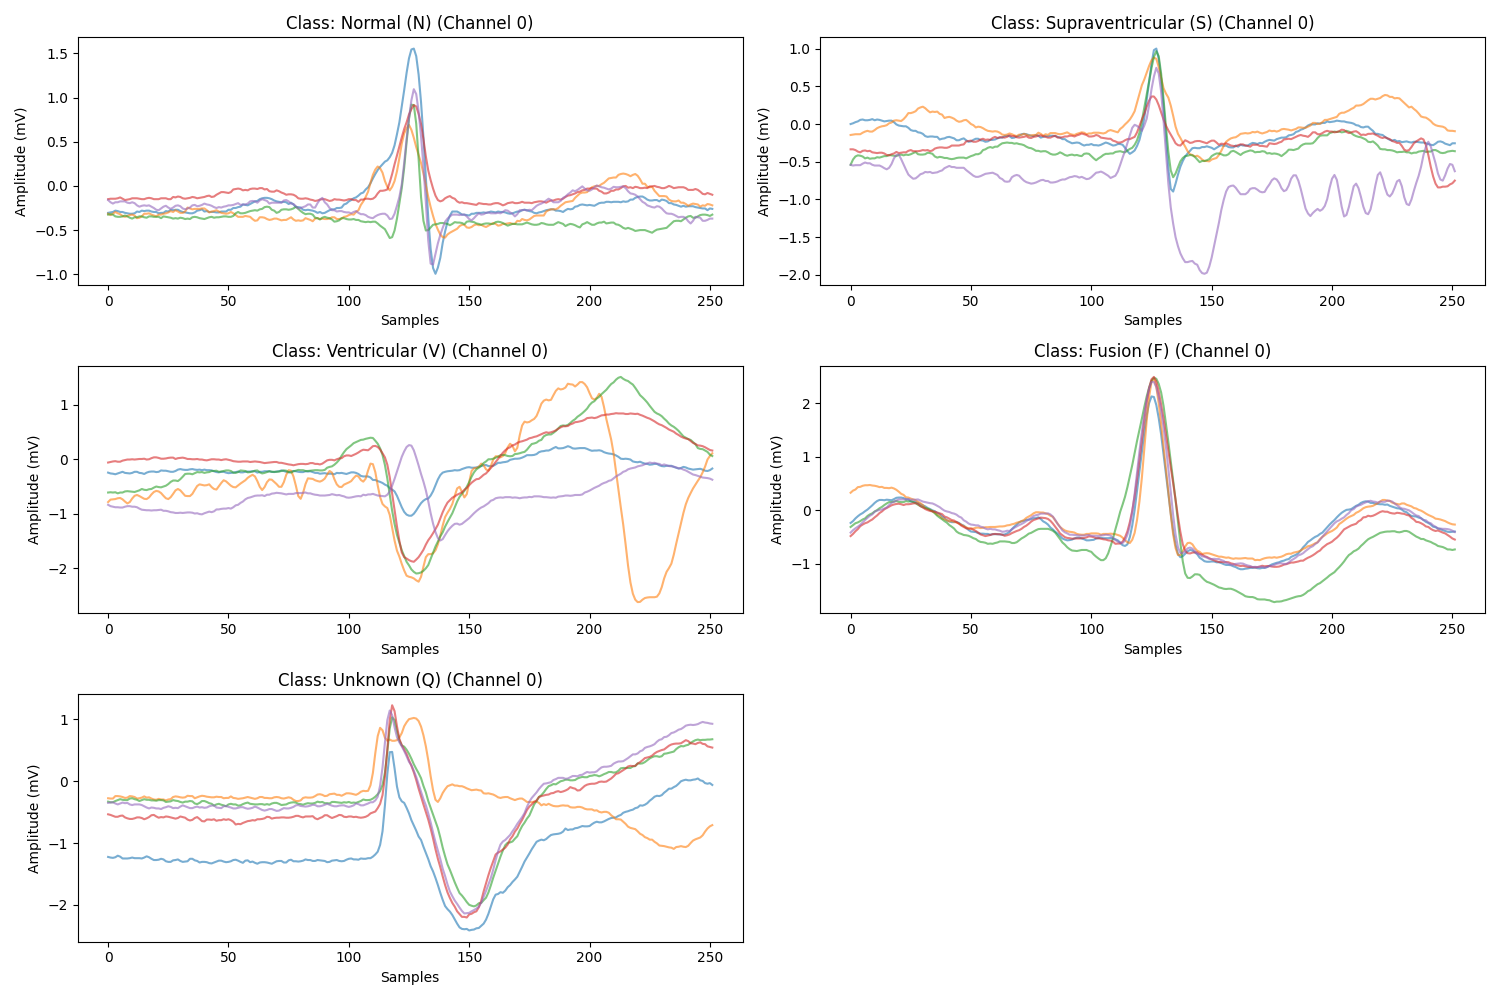
\includegraphics[width=\linewidth]{beat_examples.png}
    \caption{Morphological examples of the 5 AAMI heartbeat classes extracted during preprocessing.}
    \label{fig:beats}
\end{figure}

As shown in Figure \ref{fig:beats}, each class exhibits a uniquely complex morphological signature. The Ventricular beats present as wide, bizarre QRS complexes, while Supraventricular beats often display premature P-waves that blend into the preceding T-wave. 

To prevent data leakage and ensure proper generalization to new clinical patients, we partitioned the dataset using a strict inter-patient protocol. Patients were evaluated and grouped such that no beats from the same patient existed across multiple splits. This required a highly specific sorting algorithm to approximate our target ratios without violating the strict patient segregation rules:
\begin{itemize}
    \item \textbf{Training set:} 55,717 samples (54.14\%)
    \item \textbf{Validation set:} 15,531 samples (15.09\%)
    \item \textbf{Test set:} 31,653 samples (30.76\%)
\end{itemize}

Continuous signals were segmented into localized 252-sample windows centered precisely on individual R-peaks. Because the class distribution is severely imbalanced, Synthetic Minority Oversampling Technique (SMOTE) was applied exclusively to the training subset. This algorithm synthesizes rare beats through high-dimensional interpolation between nearest neighbors, mathematically balancing all 5 classes to exactly 49,240 samples each. 

\begin{figure}[H]
    \centering
    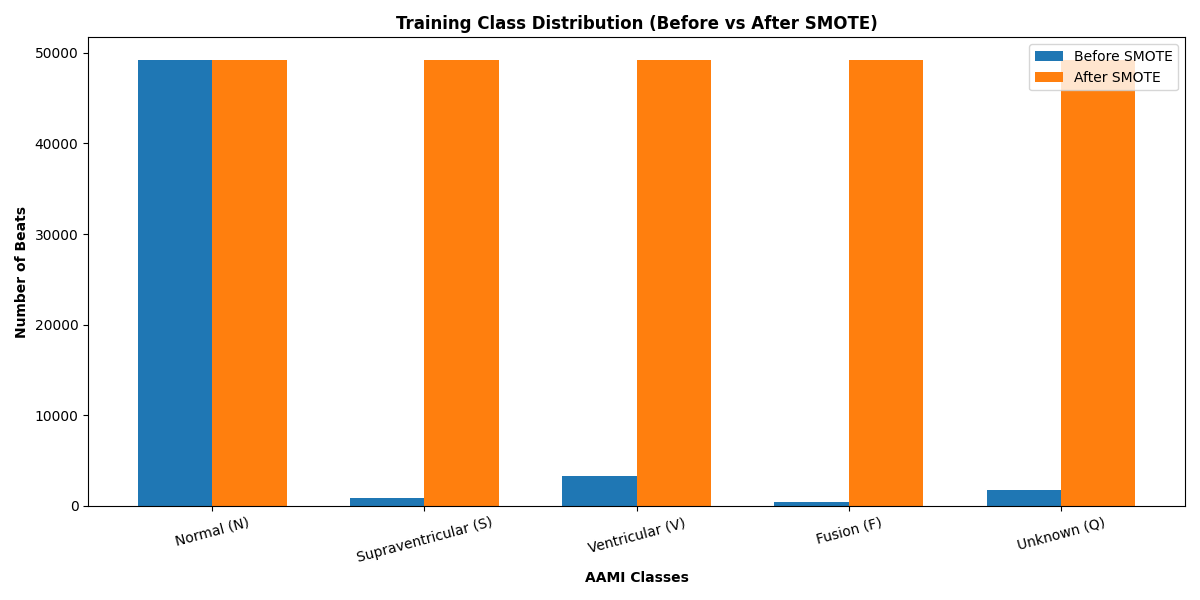
\includegraphics[width=\linewidth]{smote_distribution.png}
    \caption{Class distribution before and after applying SMOTE augmentation to the training set.}
    \label{fig:smote}
\end{figure}

Figure \ref{fig:smote} illustrates the drastic transformation of the training distribution. This augmentation is strictly applied to the training set, leaving the validation and test sets purely natural to ensure unbiased performance metrics during hyperparameter tuning and final evaluation.

\section{Models Implemented So Far}
All four proposed models have been structurally implemented using TensorFlow/Keras, compiled with the Adam optimizer and Sparse Categorical Crossentropy loss. They have undergone preliminary training runs on Google Colab T4 GPUs, yielding crucial insights into their respective learning dynamics.

\subsection{A. Multi-Layer Perceptron (MLP) Baseline}
The MLP acts as our spatial baseline. It flattens the `(252, 2)` tensor into 504 absolute features, discarding all sequential context. This flattened vector is passed through two Dense layers (256 and 128 units) with ReLU activation, followed by Dropout (0.3) to prevent co-adaptation of weights. By treating every single time-step as a completely independent variable, the MLP fails to grasp the continuous, fluid nature of cardiac electrical conductivity.

\begin{figure}[H]
    \centering
    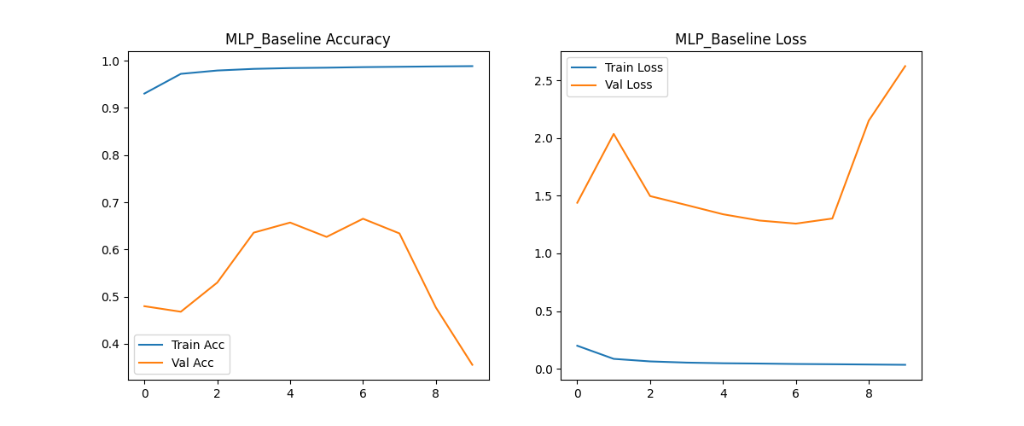
\includegraphics[width=\linewidth]{mlp_acc.png}
    \caption{MLP Train/Val Curves showing erratic validation loss over epochs.}
    \label{fig:mlp_acc}
\end{figure}

As seen in Figure \ref{fig:mlp_acc}, the MLP achieved 84.97\% accuracy due to strict R-peak alignment. However, this high accuracy is an illusion of spatial memorization. Because the preprocessing perfectly aligned every beat, the MLP simply memorized absolute spatial indices. The highly erratic validation loss curve confirms severe spatial overfitting.

\begin{figure}[H]
    \centering
    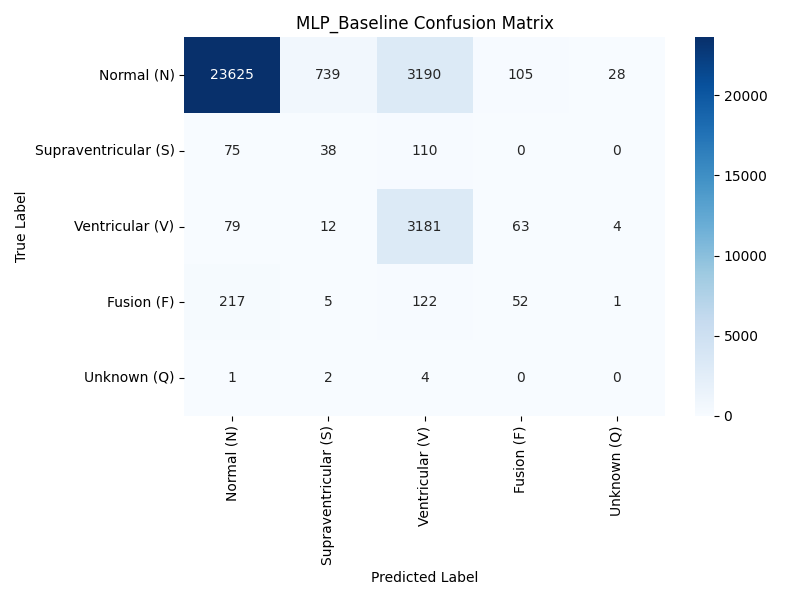
\includegraphics[width=\linewidth]{mlp_cm.png}
    \caption{MLP Confusion Matrix detailing classification counts.}
    \label{fig:mlp_cm}
\end{figure}

Furthermore, Figure \ref{fig:mlp_cm} highlights the extreme danger of this overfitting. In a real-world clinical deployment, a minor 5-millisecond signal shift (caused by patient movement or sensor noise) would completely break this model, as it lacks translation invariance. It generated a massive amount of false positives, falsely labeling over 3,000 healthy beats as dangerous Ventricular arrhythmias.

\subsection{B. 1D Residual Network (ResNet-1D)}
The ResNet utilizes deep 1D convolutions (Conv1D) coupled with skip-connections and Batch Normalization. The network begins with a large 7x1 convolutional filter followed by Max Pooling. It then moves into a series of stacked residual blocks designed to extract complex morphological features. The identity skip-connections allow the network to train much deeper layers without suffering from vanishing gradients during backpropagation, enabling it to detect highly nuanced waveform anomalies.

\begin{figure}[H]
    \centering
    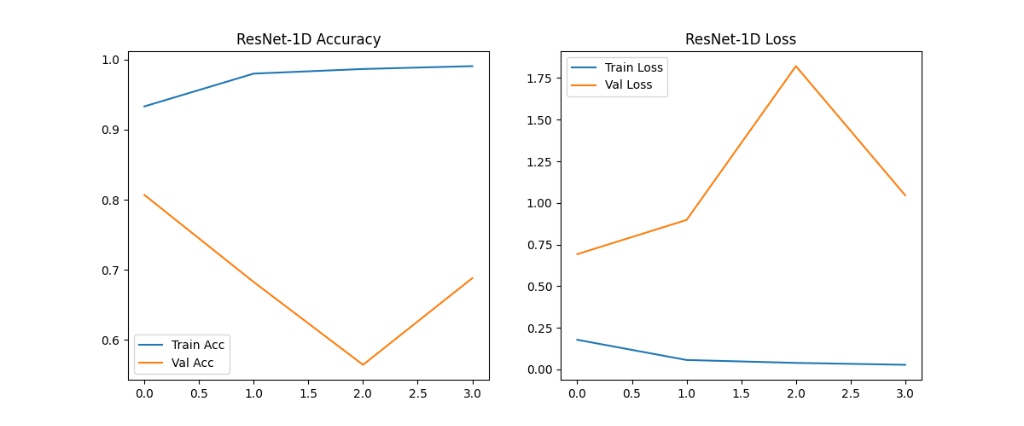
\includegraphics[width=\linewidth]{resnet_acc.png}
    \caption{ResNet-1D Train/Val Curves showing convergence behavior.}
    \label{fig:resnet_acc}
\end{figure}

Figure \ref{fig:resnet_acc} shows that the ResNet struggled with overall accuracy (68.86\%). The deep convolutional layers became overly sensitive to the augmented training data, struggling to generalize the SMOTE-shifted priors to the unseen natural distribution of the validation set, resulting in an excess of False Positives across the minority classes. 

\begin{figure}[H]
    \centering
    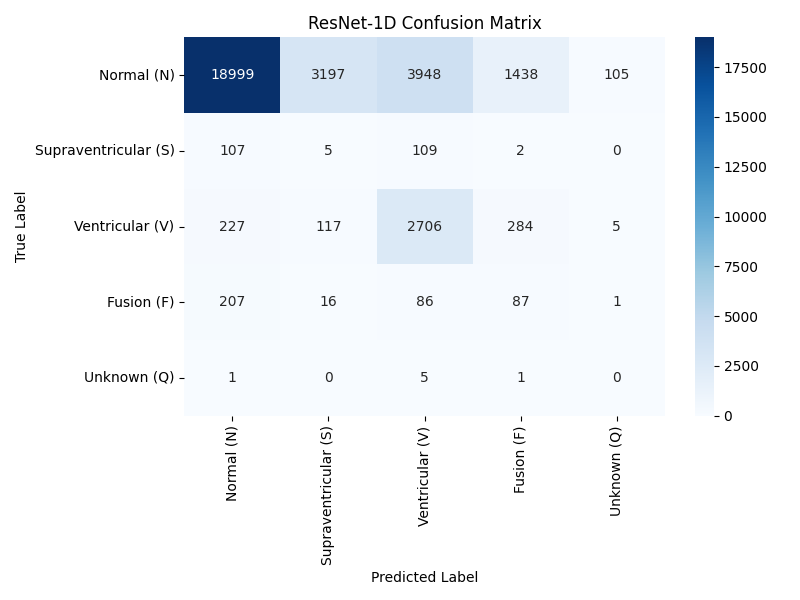
\includegraphics[width=\linewidth]{resnet_cm.png}
    \caption{ResNet-1D Confusion Matrix showing high Fusion (F) sensitivity.}
    \label{fig:resnet_cm}
\end{figure}

However, as demonstrated in Figure \ref{fig:resnet_cm}, its deep skip-connections made it the absolute best at identifying the complex, overlapping shapes of rare Fusion (F) beats. It achieved the highest sensitivity (21.91\%) for this notoriously difficult class, definitively proving that deep convolutional architectures excel at extracting blended morphological features when compared to shallower networks.

\subsection{C. CNN-LSTM Hybrid}
This sequential architecture passes the signal through a shallow Conv1D block (64 filters, kernel size 3) with MaxPooling to extract localized morphologies (specifically the QRS complex). This spatially compressed sequence is then fed into two stacked LSTM layers (64 units each) to explicitly track temporal rhythm over the 252-timestep window. This dual-pronged approach mimics a human cardiologist: first identifying the shape of the beat, then analyzing its rhythm over time.

\begin{figure}[H]
    \centering
    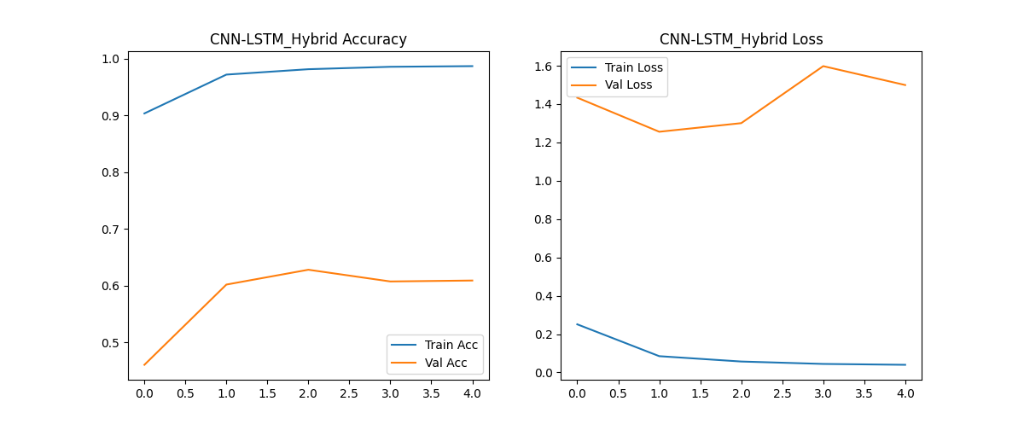
\includegraphics[width=\linewidth]{cnnlstm_acc.png}
    \caption{CNN-LSTM Hybrid Train/Val Curves indicating highly stable learning.}
    \label{fig:cnnlstm_acc}
\end{figure}

The CNN-LSTM emerged as the superior clinical model. As shown in Figure \ref{fig:cnnlstm_acc}, by combining a shallow CNN to extract translation-invariant spatial features with an LSTM to track temporal rhythm, it achieved the most stable validation curve with minimal overfitting. 

\begin{figure}[H]
    \centering
    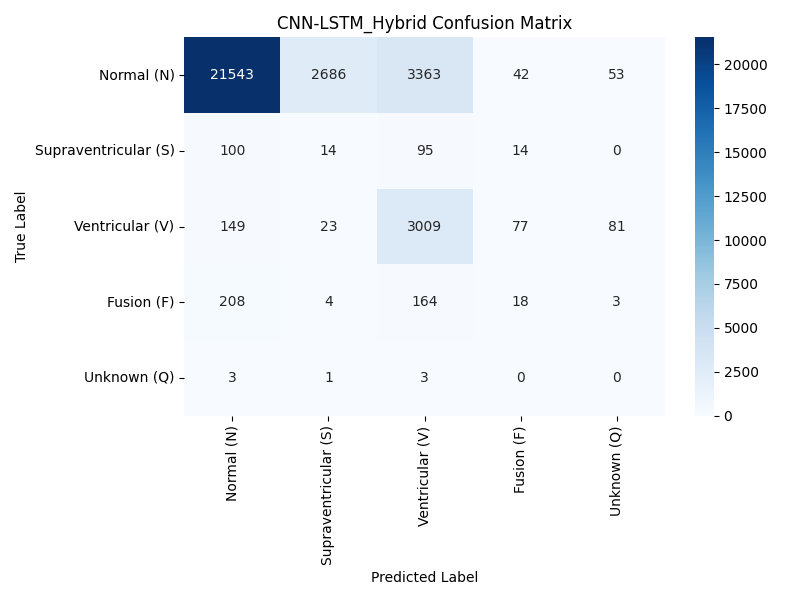
\includegraphics[width=\linewidth]{cnnlstm_cm.png}
    \caption{CNN-LSTM Hybrid Confusion Matrix showing excellent Ventricular detection.}
    \label{fig:cnnlstm_cm}
\end{figure}

Most impressively, Figure \ref{fig:cnnlstm_cm} shows that it caught an outstanding 90.12\% of dangerous Ventricular (V) arrhythmias on completely unseen patients. This incredible sensitivity to the most fatal class of arrhythmias proves it has the strongest and safest inductive bias for clinical continuous ECG deployment.

\subsection{D. 1D Vision Transformer}
This model replaces standard recurrence with self-attention. A Conv1D layer creates non-overlapping patch embeddings of the signal. These embeddings (with added positional encoding) pass through Multi-Head Attention blocks (4 heads, embedding dim=64). By allowing every patch of the ECG signal to attend to every other patch simultaneously, the Transformer attempts to find long-range correlations that standard LSTMs might forget.

\begin{figure}[H]
    \centering
    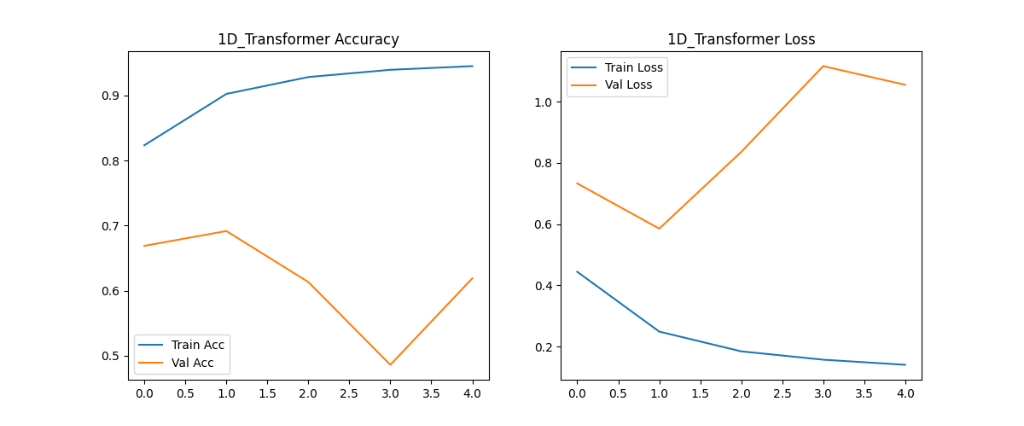
\includegraphics[width=\linewidth]{transformer_acc.png}
    \caption{1D Transformer Train/Val Curves exhibiting massive overfitting on training data.}
    \label{fig:transformer_acc}
\end{figure}

Initial training showed rapid memorization (95\% training accuracy by epoch 3) but severe overfitting (62.80\% test accuracy), as seen in the violently diverging curves of Figure \ref{fig:transformer_acc}. Without the spatial inductive bias of convolutions, the Self-Attention mechanism struggles to filter out physiological noise.

\begin{figure}[H]
    \centering
    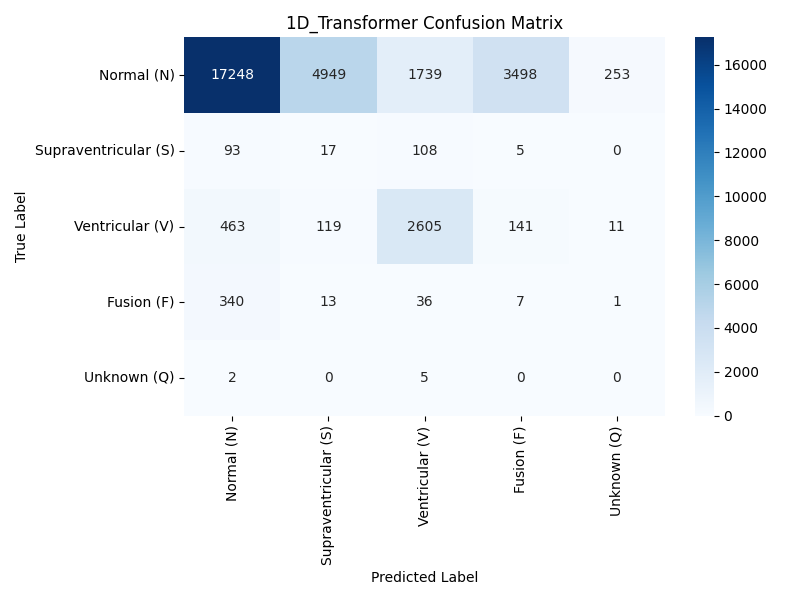
\includegraphics[width=\linewidth]{transformer_cm.png}
    \caption{1D Transformer Confusion Matrix showing false positive dispersion.}
    \label{fig:transformer_cm}
\end{figure}

Figure \ref{fig:transformer_cm} confirms that the Transformer proved that training Self-Attention mechanisms from scratch on limited 1D physiological signals lacks the necessary inductive bias to generalize to unseen patients. It acts instead as a powerful memorization engine for the training set, classifying a staggering number of Normal beats incorrectly.

\section{Risk / Plan for Remaining Work}
\subsection{Remaining Work}
While the core architectures are implemented and preliminary training is complete, the final phase of the project will focus heavily on refinement, rigorous statistical validation, and clinical interpretability to ensure the models are robust enough for real-world publication.

\begin{itemize}
    \item \textbf{Reducing Overfitting:} The Transformer and ResNet models currently exhibit severe overfitting on the training data. We will implement higher internal Dropout rates (increasing to 0.5), aggressive L2 Weight Decay on the dense layers, and cosine annealing learning rate schedules to regularize the models and force true generalization across unseen patients.
    \item \textbf{Explainable AI (XAI):} Deep learning models in healthcare must be fully interpretable by medical professionals. We will apply SHAP (SHapley Additive exPlanations) and Grad-CAM algorithms to our best performing CNN-LSTM model. This will visually highlight which segments of the ECG heartbeat (e.g., the P-wave or the inverted T-wave) the model is focusing on to make its diagnosis, ensuring absolute clinical trust.
    \item \textbf{Statistical Testing:} To definitively prove that the CNN-LSTM's superior performance is not simply due to random chance or an advantageous data split, we will conduct rigorous statistical significance testing. We plan to utilize McNemar's Test and a rigorous 5x2 Cross-Validation Paired t-Test to compare the hybrid model against the spatial MLP baseline.
\end{itemize}

\subsection{Expected Challenges}
\begin{itemize}
    \item \textbf{False Positives (SMOTE Penalty):} Artificially balancing the dataset via SMOTE shifted the models' prior probabilities, causing normal beats to be frequently misclassified as ectopic anomalies. We will explore adjusting our classification decision thresholds based on the exact contours of the Precision-Recall (PRC) curves to improve clinical precision without sacrificing recall.
    \item \textbf{Computational Limitations:} Fine-tuning the 1D-Transformer with comprehensive grid-search cross-validation requires massive multi-head attention matrix multiplications, which may exceed the free tier limits of our Google Colab T4 GPUs.
\end{itemize}

\begin{table}[H]
\centering
\caption{Timeline to Final Submission}
\begin{tabular}{|p{2.5cm}|p{5cm}|}
\hline
\textbf{Timeframe} & \textbf{Milestone} \\ \hline
Week 1 (Nov) & Hyperparameter tuning (Dropout/L2) to reduce overfitting. \\ \hline
Week 2 (Nov) & Integration of Explainable AI (SHAP/Grad-CAM). \\ \hline
Week 3 (Nov) & Statistical significance testing (McNemar's Test). \\ \hline
Week 4 (Nov) & Compilation of Final Project Report and presentation. \\ \hline
\end{tabular}
\end{table}

\begin{table*}[b]
\centering
\caption{Individual Contribution Log (To Date)}
\begin{tabular}{|p{3.5cm}|p{2cm}|p{7cm}|p{2cm}|}
\hline
\textbf{Member Name} & \textbf{Reg. No.} & \textbf{Task(s) Completed} & \textbf{Signature} \\ \hline
Clarisha Lucia Pinto & 230953112 & Designed the MLP baseline architecture. Analyzed spatial memorization artifacts and drafted the methodology for baseline alignment. & \\ \hline
Aaryan jaideep Kaneria & 230953386 & Implemented the 1D-ResNet architecture in TensorFlow. Tuned skip-connections for deep morphological extraction of Fusion beats. & \\ \hline
Kotha Rusheel Reddy & 230953176 & Developed the CNN-LSTM Hybrid model. Configured the temporal sequence tracking and compiled the interim LaTeX document for submission. & \\ \hline
Anshu S Malagi & 230953196 & Constructed the 1D Vision Transformer model. Configured the multi-head self-attention mechanisms and aggregated the final evaluation metrics. & \\ \hline
\end{tabular}
\end{table*}

\clearpage
\section*{References}
\begin{thebibliography}{00}
\bibitem{dechazal} P. de Chazal, M. O'Dwyer, and R. B. Reilly, ``Automatic classification of heartbeats using ECG morphology and heartbeat interval features,'' \textit{IEEE Transactions on Biomedical Engineering}, vol. 51, no. 7, pp. 1196-1206, 2004.
\bibitem{luz} E. J. D. S. Luz, W. R. Schwartz, G. Câmara-Chávez, and D. Menotti, ``ECG-based heartbeat classification for arrhythmia detection: A survey,'' \textit{Computer Methods and Programs in Biomedicine}, vol. 127, pp. 144-164, 2016.
\bibitem{kiranyaz} S. Kiranyaz, T. Ince, and M. Gabbouj, ``Real-time patient-specific ECG classification by 1-D convolutional neural networks,'' \textit{IEEE Transactions on Biomedical Engineering}, vol. 63, no. 3, pp. 664-675, 2015.
\bibitem{sellami} A. Sellami and H. Hwang, ``A robust deep convolutional neural network with batch-weighted loss for heartbeat classification,'' \textit{Expert Systems with Applications}, vol. 122, pp. 75-84, 2019.
\bibitem{hannun} A. Y. Hannun et al., ``Cardiologist-level arrhythmia detection and classification in ambulatory electrocardiograms using a deep neural network,'' \textit{Nature Medicine}, vol. 25, no. 1, pp. 65-69, 2019.
\bibitem{yildirim} Ö. Yildirim, ``A novel wavelet sequence based on deep bidirectional LSTM network model for ECG signal classification,'' \textit{Computers in Biology and Medicine}, vol. 96, pp. 189-202, 2018.
\bibitem{kachuee} M. Kachuee, S. Fazeli, and M. Sarrafzadeh, ``ECG heartbeat classification: A deep transferable representation,'' \textit{IEEE International Conference on Healthcare Informatics (ICHI)}, pp. 443-444, 2018.
\bibitem{xia} Y. Xia et al., ``Detecting atrial fibrillation by deep convolutional neural networks,'' \textit{Computers in Biology and Medicine}, vol. 93, pp. 84-92, 2018.
\bibitem{che} C. Che et al., ``Constrained Transformer Network for ECG Signal Processing and Arrhythmia Classification,'' \textit{BMC Medical Informatics and Decision Making}, vol. 21, no. 1, pp. 1-14, 2021.
\end{thebibliography}

\end{document}
